%----------------------------------------------------------------------------------------
%	PACKAGES AND THEMES
%----------------------------------------------------------------------------------------

\documentclass[aspectratio=169]{beamer}

\mode<presentation> {

\usetheme{Madrid}

%\setbeamertemplate{footline} % To remove the footer line in all slides uncomment this line
%% \setbeamertemplate{footline}[page number] % To replace the footer line in all slides with a simple slide count uncomment this line

\setbeamertemplate{navigation symbols}{} % To remove the navigation symbols from the bottom of all slides uncomment this line
}

\usepackage{graphicx} % Allows including images
\usepackage{booktabs} % Allows the use of \toprule, \midrule and \bottomrule in tables

%% Bunch of stuff to make a flowchart with tikz
\usepackage{tikz}
\usetikzlibrary{shapes.geometric,backgrounds,positioning,
  positioning-plus,node-families,calc}
\tikzset{
  basic box/.style = {
    shape = rectangle,
    align = center,
    draw  = #1,
    fill  = #1!25,
    rounded corners},
  header node/.style = {
    Minimum Width = header nodes,
    font          = \strut\Large\ttfamily,
    text depth    = +0pt,
    fill          = white,
    draw},
  header/.style = {%
    inner ysep = +1.5em,
    append after command = {
      \pgfextra{\let\TikZlastnode\tikzlastnode}
      node [header node] (header-\TikZlastnode) at (\TikZlastnode.north) {#1}
      node [span = (\TikZlastnode)(header-\TikZlastnode)]
        at (fit bounding box) (h-\TikZlastnode) {}
    }
  },
  hv/.style = {to path = {-|(\tikztotarget)\tikztonodes}},
  vh/.style = {to path = {|-(\tikztotarget)\tikztonodes}},
}

%----------------------------------------------------------------------------------------
%	TITLE PAGE
%----------------------------------------------------------------------------------------

\title[Summary Presentation]{Geoff Rosenberg Interview} % The short title appears at the bottom of every slide, the full title is only on the title page

\author{Geoff Rosenberg} % Your name
\institute[] % Your institution as it will appear on the bottom of every slide, may be shorthand to save space
{
%% \medskip
\textit{Geoff.Rosenberg@gmail.com} % Your email address
}
\date{June 1, 2018} % Date, can be changed to a custom date

\begin{document}

\begin{frame}
\titlepage % Print the title page as the first slide
\end{frame}

\begin{frame}
\frametitle{Overview} % Table of contents slide, comment this block out to remove it
\tableofcontents % Throughout your presentation, if you choose to use \section{} and \subsection{} commands, these will automatically be printed on this slide as an overview of your presentation
\end{frame}

%----------------------------------------------------------------------------------------
%	PRESENTATION SLIDES
%----------------------------------------------------------------------------------------

%------------------------------------------------
\section{Personal Summary} % Sections can be created in order to organize your presentation into discrete blocks, all sections and subsections are automatically printed in the table of contents as an overview of the talk
%------------------------------------------------

%% ** First 20 minutes of the presentation should be a high level overview of myself -- call it a personal statement.
%% *** Questions I want to answer
%% **** Why did I choose my schools and degrees?
%% ***** Although UW as actually the first school that I heard back from, I chose San Diego for undergrad because it made more financial sense.
%% ***** USC because it has a highly rated MS program for dynamics and controls
%% **** Why am I changing jobs?
%% ***** I've always wanted to work in space
%% ***** Don't really like working for the government and having our technology being integrated by a third party

\subsection{Goals}
\begin{frame}
  \frametitle{Overarching Mission}
  In essence, I want to go into the space industry it's because I want the world to benefit from the work I do.  That's why I went into renewable energy, and that's why I want to go into the space industry.
\end{frame}

\begin{frame}
  \frametitle{Interests} 
  \begin{itemize}
  \item I've always loved learning about how things work,
    and solving problems.
  \item Control of autonomous systems (built robots as a kid).
  \item Control software.
  \item Designing and building experiments.
  \item Won our team robotics competition at UCSD.
  \item Built estes rockets as a kid and demoed them for my 5th grade class.
  \end{itemize}
\end{frame}

\begin{frame}
  \frametitle{Motivation}
  This is where I'd like to mention that I love
  space travel and \textbf{why}.
  %% TODO I should mention that I think it's the challenge of our time/important for humanity's survival
  %% Box on the Fermi Paradox
  
  
\end{frame}

\begin{frame}
  \frametitle{Building Rockets}
  %% Show a couple of the estes rockets that I built as a kid with Dad
  %% eggspress
  %% Demoed one of these at school and built them in ELP
  
  %% \begin{itemize}
  %%   \item 
  %% \end{itemize}

\end{frame}

%% TODO College robotics frame here, if the video is still online at UCSD's website
%% \begin{frame}
%%   \frametitle{UCSD MAE 156 Robotics Champions}

%% \end{frame}

\subsection{Undergrad}
\begin{frame}
  \frametitle{Schools}
  \begin{itemize}
  \item Knew I wanted to be an engineer, but that's it.
  \item Should mention the schools I went to and why I chose them.
  \item Chose ME because it's interesting (I loved building dams a
    kid)
    \begin{itemize}
      \item Versatility
    \end{itemize}
  \end{itemize}

  \begin{figure}
    
\includegraphics[width=0.35\linewidth]{USC_Logo.png}
  \end{figure}

  \begin{figure}
    
\includegraphics[width=0.35\linewidth]{ucsd-athletics-logo.png}
  \end{figure}
\end{frame}

\begin{frame}
  \frametitle{Undergrad (UCSD)}
  \begin{columns}[t]            % t for top alignment, c for centered
    \column{0.45\textwidth}
  \begin{itemize}
  \item Was and is one of the top engineering programs in the country.
  \item The beach is nice, too :)
  \end{itemize}

  \column{0.65\textwidth}
  \begin{figure}
    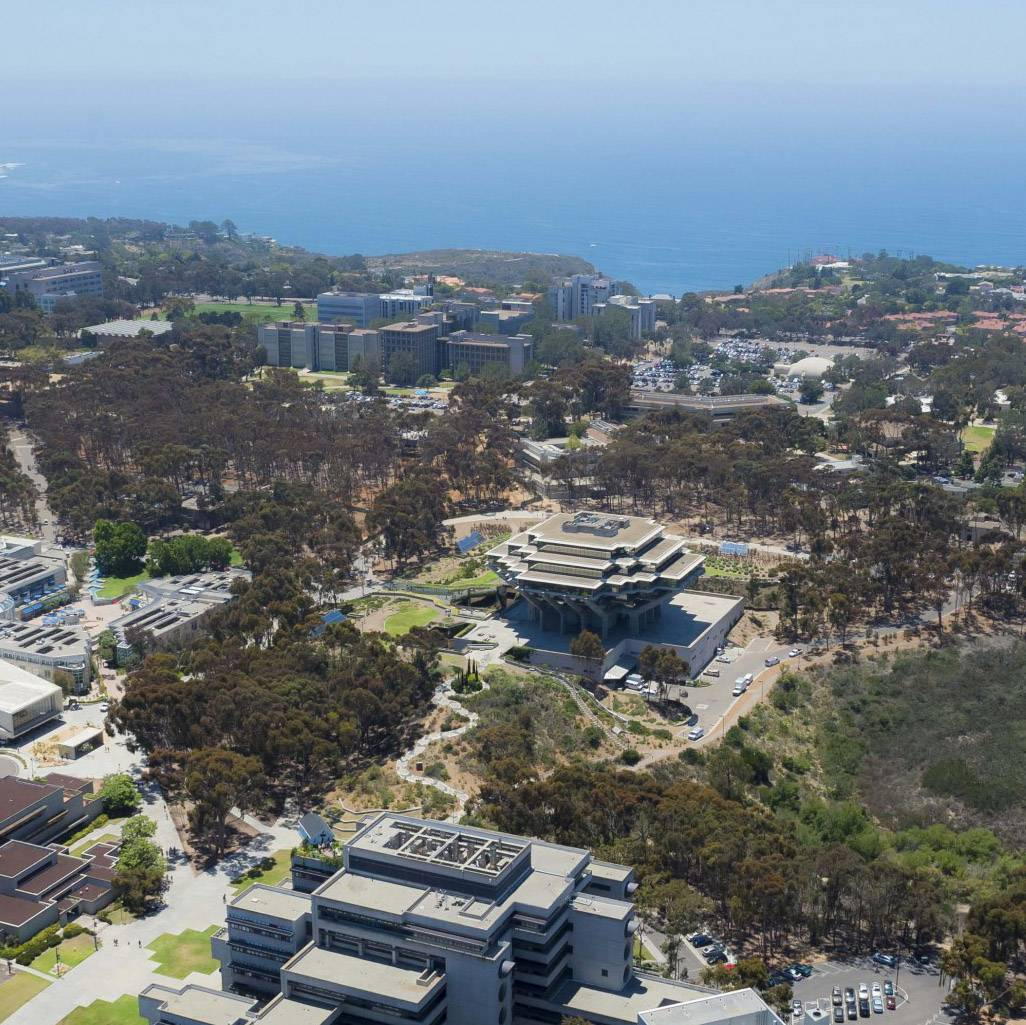
\includegraphics[width=0.7\linewidth]{UCSD.jpg}
  \end{figure}
  \end{columns}
\end{frame}

\subsection{Grad School}
\begin{frame}
  \frametitle{Grad School (USC)}
  \begin{columns}[t]
    \column{0.45\textwidth}
  \begin{itemize}
  \item I chose USC because it has a very strong dynamics and controls
    program (my favorite class during undergrad).
  \item I also got to play a lot of music.
  \end{itemize}

  \column{0.65\textwidth}
  \begin{figure}
    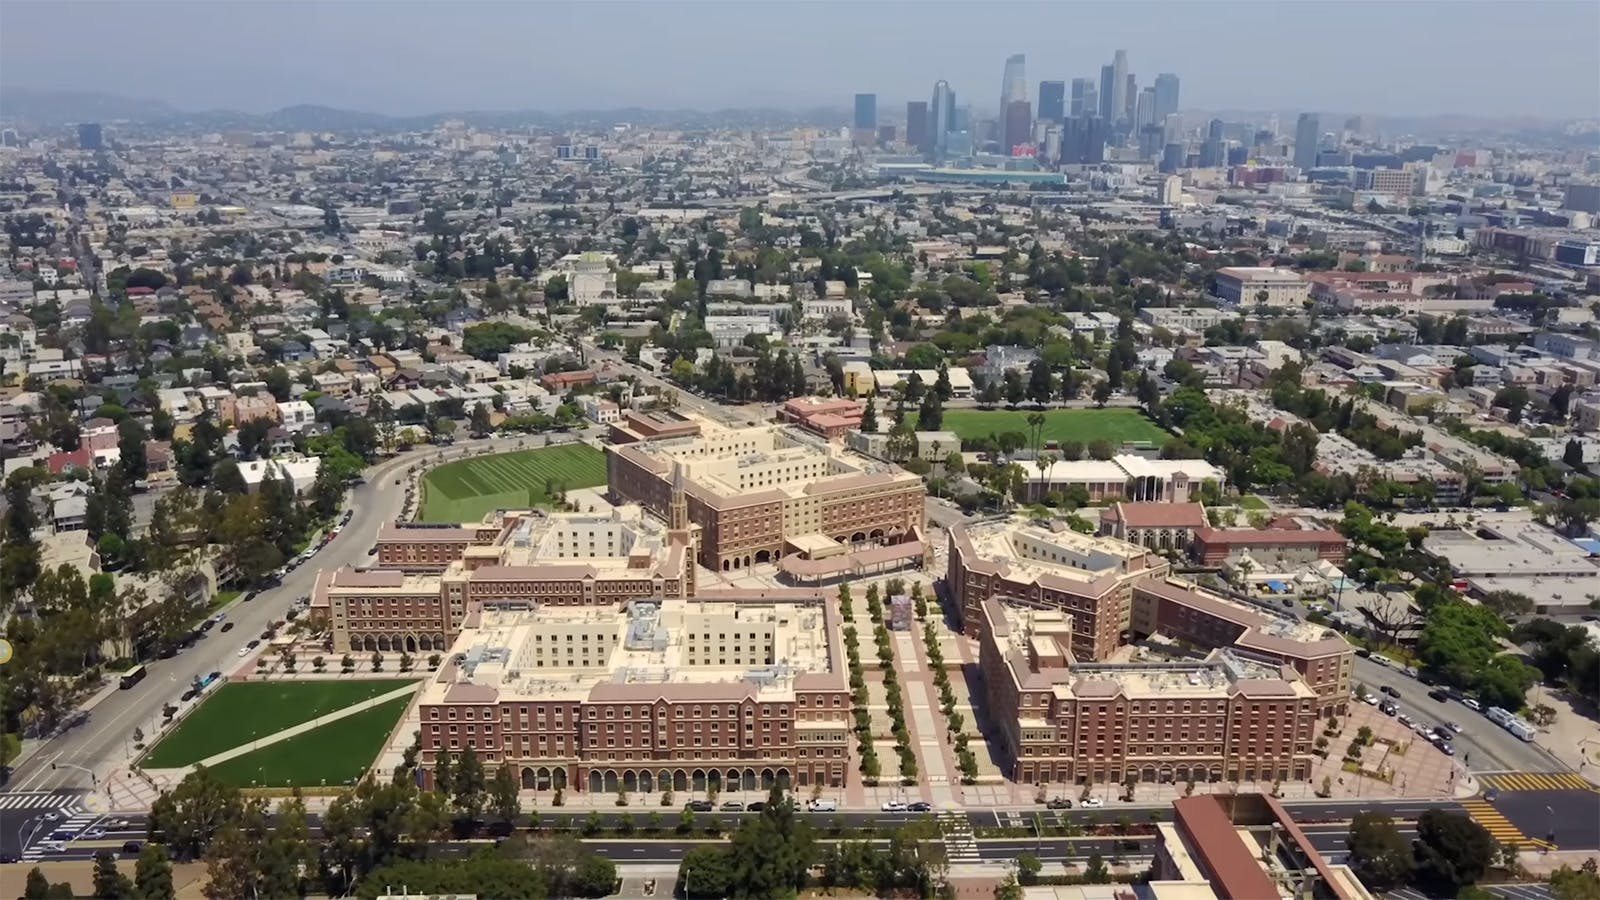
\includegraphics[width=0.7\linewidth]{USC.jpg}
  \end{figure}
  \end{columns}
\end{frame}

%------------------------------------------------
\section{Professional Career}
%------------------------------------------------

\begin{frame}
  \frametitle{Career Start -- Renewable Energy}
  %% TODO When I graduated in early 2011, the solar industry was really taking off
  % Challenging, interesting, and beneficial to the world
  
\end{frame}

\subsection{SolarReserve}
\subsubsection{Mechanical Engineer}

\begin{frame}
  \frametitle{SolarReserve}
  \center
  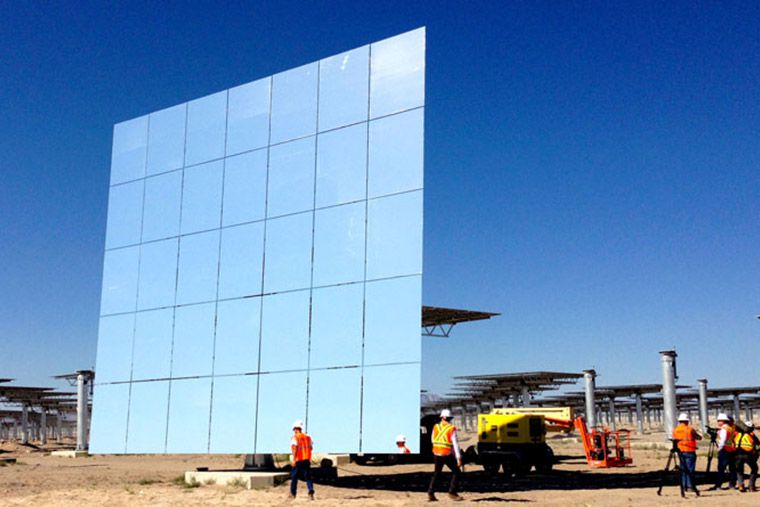
\includegraphics[width=.7\linewidth]{HeliostatImage.jpeg}
\end{frame}

%% a slide here to describe the state of the company when I joined it?
\begin{frame}
  \frametitle{SolarReserve -- Summary \& Background}
  \begin{itemize}
  \item SolarReserve was founded in 2008, primarily as power project development company rather than a technology development company
    \begin{itemize}
    \item Exclusive worldwide license to Rocketdyne's concentrated
      solar power technology
    \item Approximately tens thousand autonomously tracking solar
      mirrors (called heliostats) collect energy by heating molten
      salt.
    \item Thermal energy is collected during the day and stored, to
      be dispatched later as needed by the grid.
    \end{itemize}
  \item Joined SolarReserve in early 2011 as employee 64, one
    of few technical people at the company
    \begin{itemize}
    \item As the cognizant engineer supporting development of
      photovoltaic power projects in the US, I had to learn quickly and be resourceful. %TODO Reword
      \end{itemize}
  \end{itemize}
\end{frame}
 
\begin{frame}
  \frametitle{SolarReserve -- As A Mechanical Engineer}
  \begin{itemize}
  \item Developed a photovoltaic power plant performance toolkit.
    \begin{itemize}
    \item A PV performance model and design tool, and the systems
      engineering trades it allowed us to do it quickly.
    \end{itemize}
  \item Worked on the CDSEP plant guarantee model, integrating the
    Rocketdyne and Cobra Fortran code.
  \item Development of the CSP performance model/implementation of the
    smart dispatch logic in Matlab.
  \item Developed and debugged the PV financial model.
    \begin{itemize}
    \item I ended up learning a bit about project finance and internal
      return calculation.
    \end{itemize}
  \end{itemize}
\end{frame}

% PV performance model development slide
% Design of PV plants based on the open circuit voltage, short circuit current of the modules (show a PV IV curve to describe)
\begin{frame}
  \frametitle{SolarReserve -- Photovoltaic Design and Performance Evaluation Toolkit}
%% Two column frame
  \begin{itemize}
  \item Inputs
  \item Outputs
  \end{itemize}
\end{frame}

\begin{frame}
  \frametitle{PV System Design Tool}
  \begin{columns}[t]
    \column{0.45\textwidth}
    \begin{block}{Inputs}
      \begin{itemize}
      \item Land availability
      \item Module electrical characteristics
      \item Inverter electrical characteristics
      \item Interconnection voltage
      \end{itemize}
    \end{block}

    \column{0.45\textwidth}
    \begin{block}{Outputs}
      \begin{itemize}
      \item Overall Plant DC and AC circuit design
      \item Estimated land required
      \item Plant array capacity [MW$_{dc}$]
      \item Plant interconnection rating [MW$_{ac}$]
      \item PV module simulation software input parameters
      \item Plant output estimation time series
      \end{itemize}
    \end{block}
  \end{columns}
\end{frame}

%% Describe what knobs we have to turn in designing a plant
\begin{frame}
  \frametitle{Design Criteria for PV Plants}
  \begin{columns}[t]
    \column{0.45\textwidth}
    \begin{block}{Financial Considerations}
      \begin{itemize}
      \item Construction time \& cost
      \item Operation and maintenance costs for different tech
      \item Module cost and degradation rate
      \item Technology ``bankability''
      \end{itemize}
    \end{block}

    \column{0.45\textwidth}
    \begin{block}{Performance Considerations}
      \begin{itemize}
      \item Thin film vs monocrystalline vs polycrystalline vs CPV
      \item AC capacity (generally fixed by the interconnection agreement)
      \item Module and inverter selection
      \item Fixed tilt or tracking
      \item DC:AC Ratio
      \item Ground coverage ratio
      \item Inverter MPPT Range
      \end{itemize}
    \end{block}
  \end{columns}
\end{frame}

\begin{frame}
  \frametitle{Figures of Merit for a Candidate Configuration}
  How we characterize the ``goodness'' of a particular configuration.
  %% TODO describe why one configuration does not ``fit all''
  %% TODO Describe inverter ``clipping'' and the basics of the diurnal cycle
  
  \begin{figure}

  \begin{itemize}
  \item Annual Energy Production $\rightarrow$ From performance model.
  \item Performance Ratio $\rightarrow$ From performance model.
  \item Specific Yield $\rightarrow$ From performance model.
  \item Levelized Cost of Energy $\rightarrow$ From financial model.
    \begin{itemize}
    \item All of the above items are inputs for the project financial model.
    \end{itemize}
  \end{itemize}
    
    \center
    $NPV=\displaystyle\sum\limits_{t=0}^N\frac{R_{t}}{(1+d)^t}$
  \end{figure}
  \begin{figure}
    \raggedright
    \scriptsize
    $R_{t}$ - Net cash flow at time $t$\\
    $d$ - Discount rate\\
    $t$ - Time of the cash flow
  \end{figure}
\end{frame}

\begin{frame}
  \frametitle{Utility Photovoltaic Overview}
  %% TODO a brief frame to describe the high level components of a PV plant
  %% DC side -- Modules and associated hardware
  %% AC side -- Inverters, medium voltage transformers, GSU (high voltage) transformer
  %% hopefully find an image that shows all of these components
\end{frame}

\begin{frame}
  \frametitle{Configuring the DC System}
  \begin{block}{Electrical Requirements}
    \begin{columns}
      \column{0.45\textwidth}
      \begin{itemize}
      \item The DC side of a photovoltaic plant block is configured
        with $n$ parallel strings of $m$ modules in series.
      \item Module $I_{max} * n <$ Inverter's DC bus current rating
        $\rightarrow$ driver for $n$
      \item Module $V_{max} * m <$ Inverter's DC bus voltage rating
        $\rightarrow$ driver for $m$
      \end{itemize}

      \column{0.45\textwidth}
      \begin{figure}
        \textbf{Module Current/Voltage Relationship}
        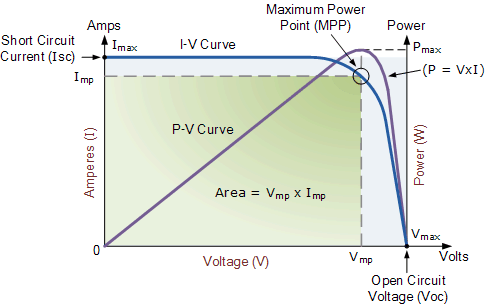
\includegraphics[width=0.75\linewidth]{IV_Curve.png}
      \end{figure}
    \end{columns}
  \end{block}
  \begin{block}{Land Usage Requirements}
    \begin{itemize}
    \item Trade between packing modules closer together to reduce land
      usage, and causing modules to shade one another at low solar
      elevation in the morning and evening.
    \item Solar trackers improve output during the morning and
      evening relative to fixed arrays, but require more space.
    \end{itemize}
  \end{block}
\end{frame}

\begin{frame}
  \frametitle{Configuring the AC System}
  \begin{columns}[t]
    \column{0.65\textwidth}
    \begin{itemize}
    \item Conversion of DC power to AC through PWM.
    \item 60 Hz sinusoid (power grid frequency) broken into multiple
      steady state DC output levels.
    \item Inverter carrier frequency of approximately 4 kHz.
    \item Selection of the minimum DC Bus voltage tracking range
      affects the AC voltage output. (Peak AC voltage = minimum DC
      tracking voltage - haircut)
    \item Design enough inverters into the plant such that there is
      enough AC capacity to cover the total output from the array
      under ideal conditions.
      \begin{itemize}
      \item Energy is wasted otherwise.
      \end{itemize}
    \end{itemize}

    \column{0.45\textwidth}
    \begin{figure}
      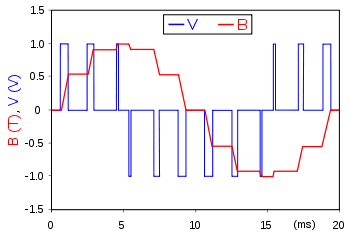
\includegraphics[width=0.75\textwidth]{PWM.png}
    \end{figure}    
  \end{columns}
\end{frame}

\begin{frame}
  \frametitle{Utility PV Inverters}
  \begin{figure}
    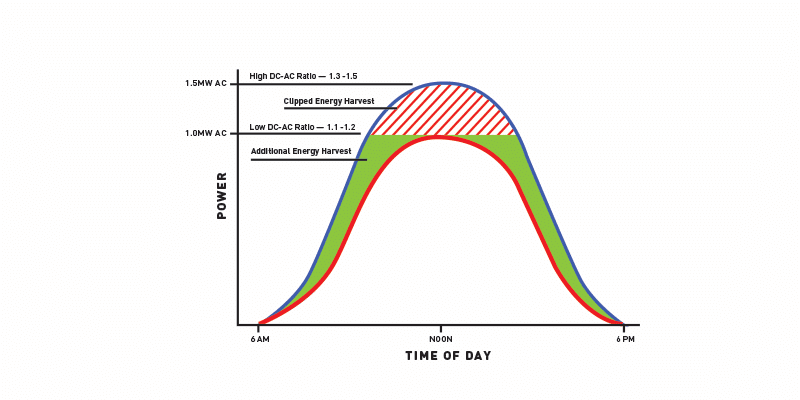
\includegraphics[width=\linewidth]{Inverter_Clipping.png}
  \end{figure}
\end{frame}

\begin{frame}
  \frametitle{Configuring Balance of Plant}
  \begin{itemize}
    \item SCADA System
    \item Tracking
  \end{itemize}
\end{frame}

\begin{frame}
  \frametitle{PV Performance Calculation}
  \begin{itemize}
    \item Interfaces with PVSyst or SAM implementations of the 6 parameter model for PV collectors (TODO Who wrote the paper?)
  \item Matlab code to handle calculation of gen tie losses based on
    power factor assumption, line impedance estimate, and
    interconnection voltage.
  \item $I^{2}Z$ losses.
  \item Optional time of day multiplier; energy delivered during peak
    demand hours is worth more to the customer.
  \item Calculation of P50, P90, and P10 annual outputs, based on
    decades of hourly solar resource data
  \item Solar resource data available since the late 1990's, thanks to the GOES satellites. %TODO: who owns the goes satellites?
  \end{itemize}
\end{frame}

%% CSP Technology overview
%% An overall flowchart would be good here.
\begin{frame}
  \frametitle{CSP Technology}
  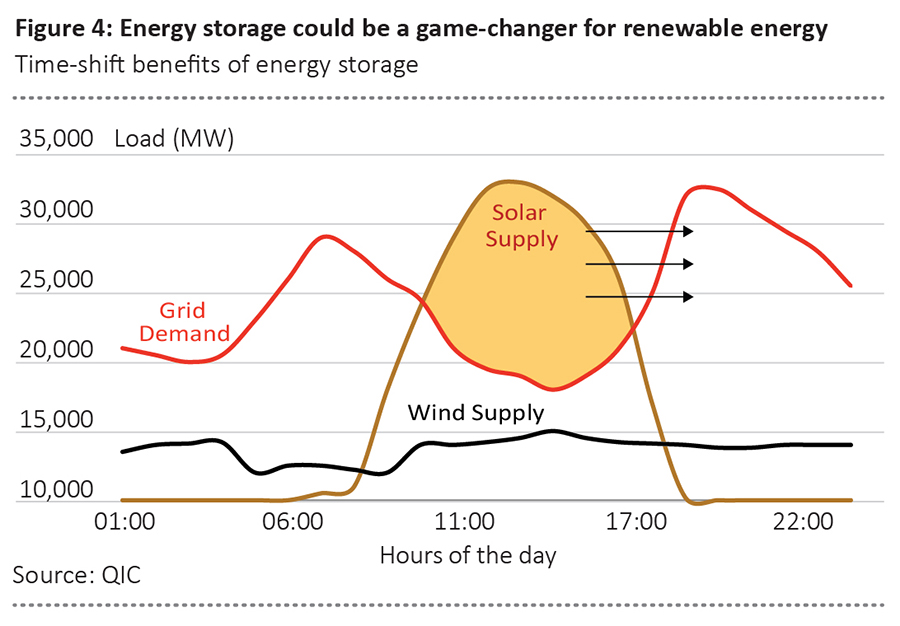
\includegraphics[width=\linewidth]{SolarEnergyStorage.jpg}
\end{frame}
  
\begin{frame}
  \frametitle{CSP Performance: Flux Model}
  Development of a Monte Carlo ray tracer to estimate the performance
  of a CSP plant's collector field based on the level of solar
  irradiation

  \begin{itemize}
  \item Vector mechanics and coordinate system transformations
  \item Written in Fortran
  \item Determine's the heliostat kinematics (drive angles and orientatons) for each heliostat in the field, and performs ray tracing
  \end{itemize}  
\end{frame}

\subsubsection{Systems Engineer}
%% All of the bullet points below deserve a slide
\begin{frame}
  \frametitle{As A Systems Engineer}
  \begin{itemize}
  \item Development of the SR-120 control software (Matlab)
  \item Kalman filter development
  \item Include some stuff about the ``zero'' finding logic?
  \item Development of the SVS-Vistek and ViewWorks camera interfaces
    in C\#
  \item Test campaigns for the SR-120
  \item Determination and definition of performance requirements (IE
    mirror slope and pointing errors)
  \item Hands on testing at Sandia National Labs
  \item Troubleshooting and modifying the AMS software
  \item Camera and SPCA network setup
  \item Daily SCRUMS (agile development) and piloting the system with
    Mark and Roger
  \item All of the performance data processing, which I had to
    automate because the rest of the team started on the SR-96
  \item Development of the in-situ/star characterization software
  \item Development of the control system interface; changing a
    relational object database into an object database.
  \end{itemize}
\end{frame}

%% Describe what the SR-120 is, a few of its features, and how I contributed
\begin{frame}
  \frametitle{SR-120 Heliostat Development}
  \begin{itemize}
  \item Development of a new and disruptive type of heliostat design
  \item Wireless power and communication
  \item Two orders of magnitude smaller than conventional heliostats
    \begin{itemize}
    \item On the order of one million per plant $\rightarrow$ mass
      production becomes a possibility
    \end{itemize}
  \item Optically controlled, with central camera controller in the tower
    \begin{itemize}
    \item Star communication topology
    \end{itemize}
  \end{itemize}
  My involvement on this project was chiefly the development of all software interfaces between the Matlab software and the hardware it controlled.  I was also involved in I\&T and debugging the Matlab code.
\end{frame}

%% Slide on the SR-120 software development
\begin{frame}
  \frametitle{SR-120 Heliostat Development -- Control Software}
  %% Zero finding and Kalman filter development
  %% Background of the Kelly 6 parameter model (Matt Kelly's MIT master's thesis)
    \begin{itemize}
    \item Adaptation of an MIT thesis originally for a siderostat at Mt. Wilson observatory in Los Angeles
    \item Adaptation of a 6 parameter kinematic model to describe errors in heliostat placement
    \item Computer vision code developed to reliably identify optical elements on the body of the heliostats
      \begin{itemize}
      \item Maximum likelihood estimation achieved through an extended Kalman filter
      \end{itemize}
    \item Chiefly written in Matlab, with hardware drivers written in C++/CLI and C\#
    \item Architecture involved both open loop and closed loop components to reduce communication bandwidth requirement
    \end{itemize}
\end{frame}

\begin{frame}
  \frametitle{SR-120 Heliostat Development -- Hardware Interfaces}
  %% Camera Interfaces and AMS software
    \begin{itemize}
    \item Hardware vendors typically provide a C API as an interface
    \item SR-120 software developed in object oriented Matlab
    \item I developed .NET assemblies to act as ``middleware'' between the SR-120 control software and the hardware
      \begin{itemize}
        \item Camera
        \item Heliostat control assembly hardware
      \end{itemize}
  \end{itemize}
\end{frame}

\begin{frame}
  \frametitle{In-Situ Heliostat Characterization at Crescent Dunes}
      $E_{Grid}= SolarIntensity * A_{Glass} * \eta_{CollectorField} * \eta_{Receiver} * \eta_{Rankine}$
  \begin{itemize}
  \item Development of a method to characterize heliostat performance en masse in the field.
  \item Heliostat optical performance is the main contributor to $\eta_{field}$
  \item Measurement of the ``bending'' heliostats to determine the deformation of the mirror figure and its ultimate effect on plant revenue
  \item Heliostat performance measurement using previously existing measurements was slow, error prone, and labor intensive
  \end{itemize}
\end{frame}

%% HabConnect relational database interface to write to the SCADA system's database
\begin{frame}
  \frametitle{In-Situ Characterization -- Software Development}
  \begin{itemize}
  \item Re-used large amounts of code originally developed for the SR-120
  \item CDSEP main field control system runs in GE Grid eTerra environment
    \begin{itemize}
    \item Necessitated an interface between the main plant control system's database and our Matlab software, which I wrote.
    \item Utilized GE Grid's HabConnect C API
    \end{itemize}
  \end{itemize}
\end{frame}

%% HabConnect relational database interface to write to the SCADA system's database
\begin{frame}
  \frametitle{In-Situ Characterization -- Hardware Development}
  \begin{itemize}
  \item Nighttime testing campaigns involved mounting a camera to the
    CDSEP tower at night
  \item Detachable, allowing it to be stowed during daytime operation of the plant
  \item Repeatable to sub milliradian accuracy
  \item Assembled from Thorlabs components for precision motion control
  \item Went through several desktop iterations before field testing it
  \end{itemize}
\end{frame}

%% All of the testing campaigns at SNL
\begin{frame}
  \frametitle{Integration and Test -- Sandia}
  \begin{columns}[c]
    \column{0.5\textwidth}
    \begin{figure}
      \textbf{Solar Thermal Test Facility\\Sandia National Labs
        (Albuquerque, NM)}
      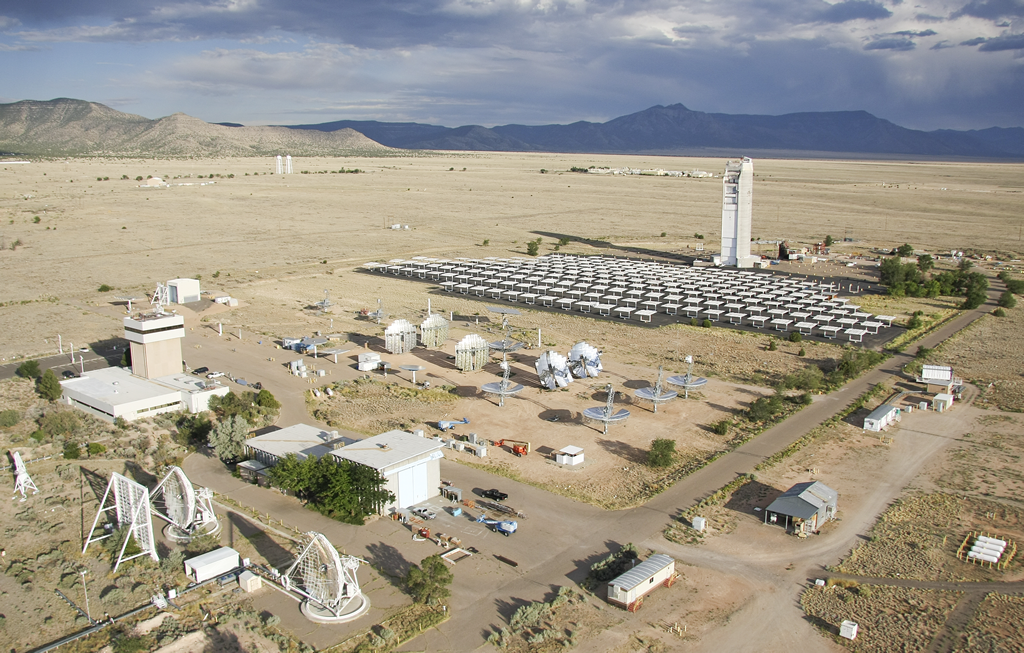
\includegraphics[width=\linewidth]{Sandia.png}
    \end{figure}

    \column{0.5\textwidth}
    \begin{itemize}
    \item Field testing of SR-120 hardware and software occurred at
      Sandia National Labs.
    \item Initial field testing of the In-Situ characterization system did as well.
    \item Much of this testing occurred remotely, controlling the hardware in Albuquerque from Santa Monica.
    \item Experiment design, and several trips over the years for field testing
    \end{itemize}
  \end{columns}
\end{frame}

\begin{frame}
  \frametitle{Integration and Test -- Crescent Dunes}
  \begin{columns}[c]
    \column{0.5\textwidth}
    \begin{figure}
      \textbf{Crescent Dunes Solar Thermal Power Plant\\
        (Tonopah, NV)}
      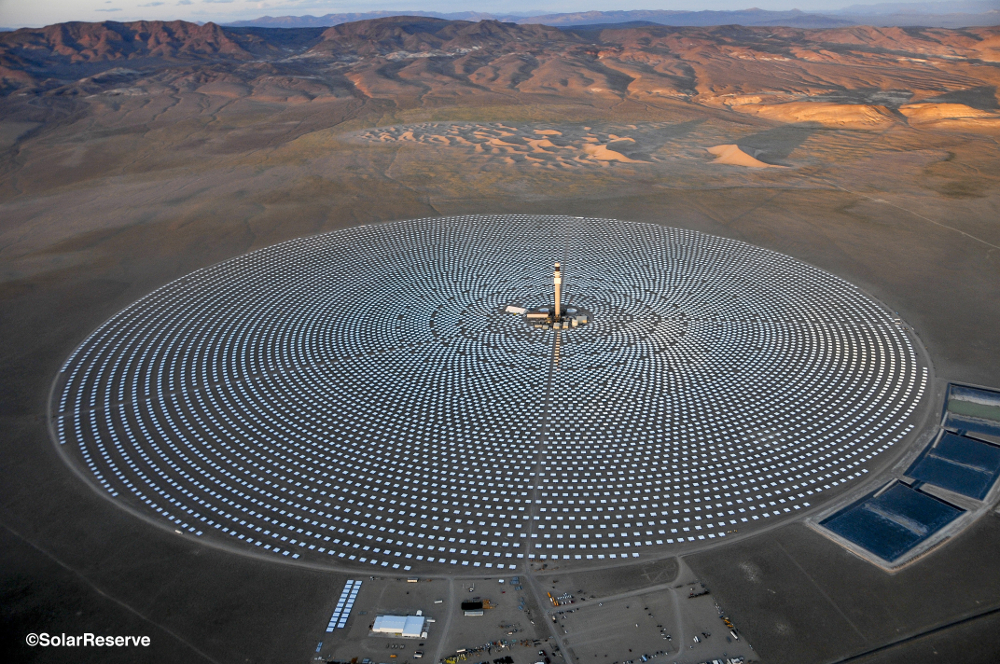
\includegraphics[width=\linewidth]{CDSEP.jpg}
    \end{figure}

    \column{0.5\textwidth}
    \begin{itemize}
    \item Most testing of the In Situ characterization software occurred at Crescent Dunes
    \item Challenges setting up the testing in an operating power
      plant/construction zone
    \end{itemize}
  \end{columns}
\end{frame}

\begin{frame}
  \frametitle{Integration and Test -- Raymer Test Facility}
  \begin{columns}[c]
    \column{0.5\textwidth}
    \begin{figure}
      \textbf{Crescent Dunes Solar Thermal Power Plant\\
        (Tonopah, NV)}
      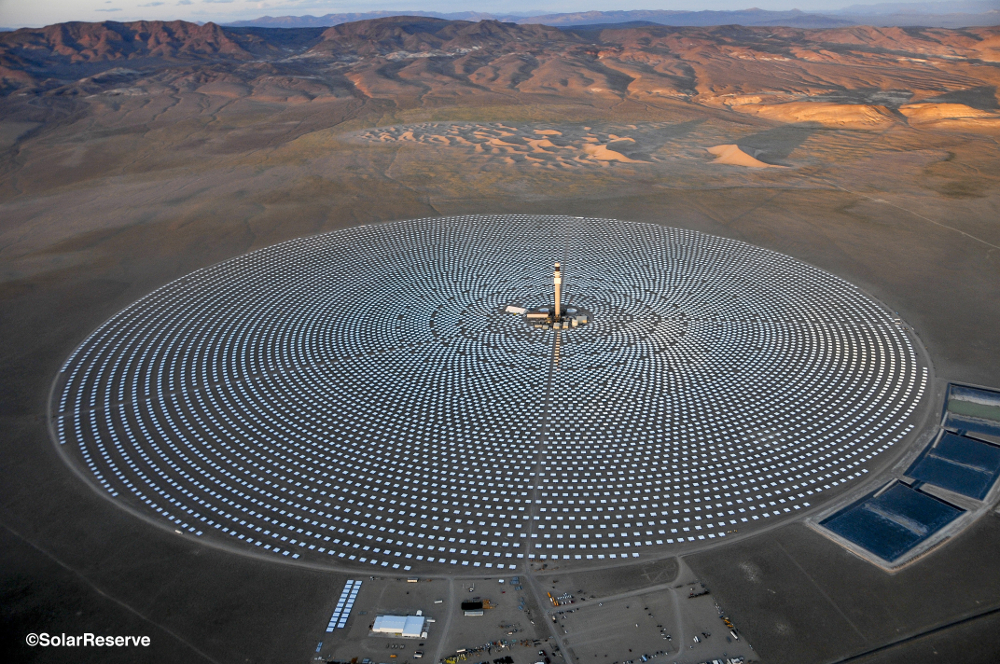
\includegraphics[width=\linewidth]{CDSEP.jpg}
    \end{figure}

    \column{0.5\textwidth}
    \begin{itemize}
    \item Description of the in-situ canting field testing
    \end{itemize}
  \end{columns}
\end{frame}

\subsection{Lockheed}
% I'm pretty sure the logo is copyrighted, so I shouldn't use it...
\begin{frame}
  \frametitle{Lockheed Martin Missiles and Fire Control}
  \center
  
\includegraphics[width=.7\linewidth]{LockheedLogo}
\end{frame}

%reasons for transition
\begin{frame}
  \frametitle{Transitioning from SolarReserve}
  \begin{itemize}
  \item Concerns about R\&D budget cuts.
  \item Concerns about being in my first job for over 6 years.
  \end{itemize}
\end{frame}

\begin{frame}
  \frametitle{Affordability Test Bed}
  \begin{itemize}
  \item Small lab at the MFC Innovation center
  \item Evaluation of COTS components and substituting them into
    existing designs
  \item Components in the lab
    \begin{itemize}
    \item Optical Bench
    \item 3D Printer
    \item Image generator
      \begin{itemize}
        \item Big computer with lots of graphics cards --
          renders images very quickly to a screen on the bench
        \item Uses a UDP client/server architecture to ensure that it
          stays ``in step'' with the running simulation
      \end{itemize}
    \item Flight computer running on a TI AM5728 chip set (Arm Cortex A15)
    \end{itemize}
  \end{itemize}
\end{frame}

\begin{frame}
  \frametitle{Loitering Munition Simulation Overview}
  %% Describe the loitering munition simulation
  %% Most of the sim and flight computer software is written in Simulink, and autocoded to c++ for deployment on a Beagleboard x15 (Arm AM5728 board with a cortex )
  %% All lower level stuff (frame handling, hardware interfaces) is written by hand in c++.  This is what I worked on.
  \begin{itemize}
  \item Continuous time simulation of a loitering munition
    \begin{itemize}
    \item Computer vision -- on board camera sends live images back to the user
    \item Simulation of a fixed wing drone with either explosives or EMP on it
    \item Semi-autonomous
      \begin{itemize}
      \item User gets the target in the camera's FOV, then designates
        it with a tablet and the autopilot takes over.
      \end{itemize}
    \end{itemize}
  \end{itemize}
    \begin{figure}
      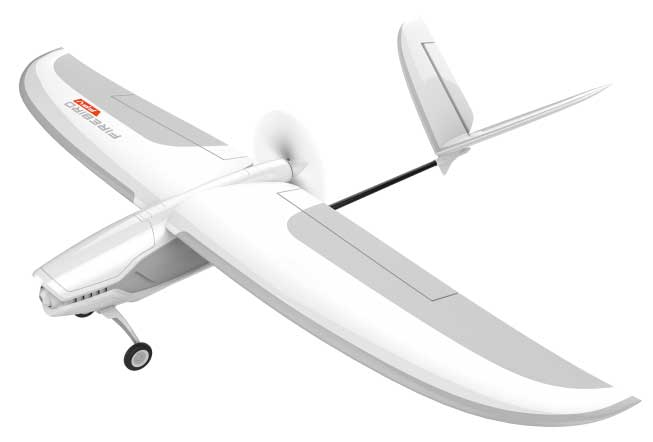
\includegraphics[width=0.4\textwidth]{Firebird-FPV-Fixed-Wing-Drone.jpg}
    \end{figure}
\end{frame}

\begin{frame}
  \frametitle {Loitering Munition Overview -- Continued}
  \begin{itemize}
  \item High level simulation and flight computer software 
  \item Written in Simulink and autocoded to C++ for deployment on a Beagleboard x15 (Arm cortex TODO number)
  \item Simulation running on a Linux PC (Redhat) host
  \item My first task -- adapted the simulation to work with a different airframe
  \item My second task -- solution of the frame delay problem
  \end{itemize}
\end{frame}

\begin{frame}
  \frametitle{Loitering Munition -- Frame Delay Problem}
  \begin{itemize}
  \item Non-zero latency between the $n^{th}$ update of the simulation state
    (simulation time $t_{n}$) and when the image is rendered on the
    screen ($t_{n+\delta}$)
  \item Causes erratic performance of the camera motion compensation
    code, which works based on TODO describe...
    \begin{itemize}
    \item This problem worsens with shorter time constant (IE faster)
      munitions
    \end{itemize}
  \end{itemize}
\end{frame}

\begin{frame}
  \frametitle{Loitering Munitions -- Frame Delay Solution}
  \begin{itemize}
    \item Software frame number overlay generation using the image generator's API with CIGI messaging
  \item Camera triggering
    \begin{itemize}
    \item Display port $\rightarrow$ DVI $\rightarrow$ HDMI
      $\rightarrow$ VGA $\rightarrow$ BNC 5 wire (RGB + HSYNC + VSYNC)
      $\rightarrow$ Alligator clips $\rightarrow$ Camera
    \end{itemize}
  \item Optical character recognition software written to read the
    frame number off the screen
  \item TODO Show the frame delay histogram (generate one
    in Python)
  \item Oscilloscope testing to determine sync pulse voltage and frequency
  \item Tested the camera's hardware triggering with a waveform generator
    before installing the hardware on the bench    
  \end{itemize}
\end{frame}

%% Image injection/projection flow charts
%define some colors for the blocks
\definecolor{light_blue}{RGB}{2,127,237}

%% color definitions for the different signals
\definecolor{Ethernet}{RGB}{5,163,0}        %green
\definecolor{HDMI}{RGB}{163,111,0}   %gold
\definecolor{USB}{RGB}{0,0,255}
\definecolor{Data}{RGB}{0,0,0}

\begin{frame}
  \frametitle{Loitering Munition -- Image Projection Data Flow}
\begin{tikzpicture}[node distance = 0.6cm, thick, nodes = {align = center},
    >=latex]
  %% simulation host
  \node[fill = light_blue] (6_DOF)
       {6DOF state @\\$t_{n}$};
  \node[fill = light_blue, below = of 6_DOF] (Cigi_Cmds)
       {Cigi Update Commands};
  \node[fill = light_blue, below = of Cigi_Cmds] (Frame_Logger)
       {Frame Logger};
  \node[fill = light_blue, below = of Frame_Logger] (PNG)
       {Images Saved as PNG};
  \node[fill = light_blue, right = of PNG] (Timestamp_Log)
       {Logging of time stamps\\and file names};
  \node[fill = light_blue, left = 1.5 of PNG] (Update_Log)
       {Cigi Update Log\\$t_n$, Frame Number};
  \node[fill = light_blue, above = 1.25 of 6_DOF] (Monitor)
       {Monitor};

  %% Image generator
  \node[fill = light_blue, left = 4 of 6_DOF] (Scene_Render)
       {Scene\\Rendering};

  %% Flight computer
  \node[fill = light_blue, right = 1.5 of Cigi_Cmds] (Image)
       {Image Received @\\$t_{n+\delta}$};
  \node[fill = light_blue, above = 1.25 of Image] (Camera)
       {Camera};

  %background nodes to separate out the computers
  \begin{scope}[on background layer]
    \node[fit = (6_DOF)(Cigi_Cmds)(Frame_Logger), basic box = red,
      header = Simulation Host] (Host) {};

    \node[fit = (Scene_Render), basic box = blue,
      header = Image Generator] (Image_Generator) {};

    \node[fit = (Image)(Camera), basic box = blue,
      header = Flight Computer] (Flight_Computer) {};
  \end{scope}

  %% paths to connect the nodes
  \path[very thick, Data] (6_DOF.south) edge[->] (Cigi_Cmds.north);
  \path[very thick, Ethernet] (Cigi_Cmds) edge[->] (Scene_Render);
  \path[very thick, Data] (Cigi_Cmds) edge[->] (Update_Log);
  \path[very thick, HDMI] (Scene_Render) edge[->] (Monitor.west);
  \path[very thick, HDMI] (Monitor.east) edge[->] (Camera.west);
  \path[very thick, USB] (Camera.south) edge[->] (Image);
  \path[very thick, Ethernet] (Image) edge[->] node[pos=0.35, sloped, above] {Image Data} (Frame_Logger);
  \path[very thick, Data] (Frame_Logger) edge[->] (Timestamp_Log);
  \path[very thick, Data] (Frame_Logger) edge[->] (PNG);
\end{tikzpicture}
\end{frame}

\begin{frame}
  \frametitle{Loitering Munition Deployment}
  %% Deployed at gifix for the army
\end{frame}

\begin{frame}
  \frametitle{IR Projector Setup}
  %test IR camera selection
  %sample pixel packing code -- knew how to do this from work at SR on cameras
\end{frame}


\begin{frame}
  \frametitle{PAC-3} % I might want to be a little sparing in my descriptions here, because this stuff is classified
  \begin{itemize}
  \item Intended to engage and destroy tactical ballistic missiles
  \item Most of it is classified
  \item Work on a Linux computing cluster on a continuous time simulation
  \item Integrating changes to the simulation from both internal, and also from the customer (IE the government), as well as the ground system components (which are from Raytheon).
  \item Integration of an older version of the simulation (entirely Fortran/Linux based) and modularizing it into several libraries which the customer can link together.
  \item Builds on Windows or Linux
  \end{itemize}
\end{frame}

\begin{frame}
  \frametitle{Configuration Management on PACNET}
  \begin{itemize}
  \item Handling configuration management on a simulation of about 800,000 SLOC
  \item Handling requests for modification
  \item Installing new releases of our code
  \item Handling updates from the system integrator
  \end{itemize}
\end{frame}

\begin{frame}
  \frametitle{Closing Comments}

\end{frame}

\begin{frame}
\Huge{\centerline{Q\&A?}}
\end{frame}

\subsection{Supplemental}

%% KSP
%% Home network & server setup
%% Electric guitar wiring
\begin{frame}
  \frametitle{Other Projects}
  \begin{itemize}
  \item Electric Guitar Wiring
  \item Home Network setup
  \item Linux Server Administration
  \end{itemize}
  
\end{frame}

\begin{frame}
  \frametitle{Electric Guitar Wiring}
  %% circuit diagram
  %% Network diagram  
\end{frame}

\begin{frame}
\frametitle{Server Administration}
\end{frame}
\end{document}
